\noindent A series of fast VCTs for specific drafting angle and test scenarios as listed in Table \ref{tab:VCT_optiwise} were conducted by Shipflow Motions. Those tests are not just used for identifying the model parameters, but also used as references for comparison of hydrodynamic forces, which are either predicted for various drift/rudder angles, or estimated by the identified model for the Optiwise experimental model tests. Rudder force predictions with the MMG original rudder model and the modified MMG quadratic model were compared to the VCT data for the rudder angle variation as shown in \autoref{fig:rudder_angle_compare_optiwise}. The newly added initial inflow angle parameter $\gamma_0$ (see \autoref{eq:gamma_R2}) allows the MMG quadratic model to have a better fit to the VCT data. The difference between the models is however less obvious when looking at the thrust variation tests in \autoref{fig:thrust_variation_optiwise}.

Furthermore, the results of drift, circle tests, circle and drifting tests are used to validate the MMG model improved by this study (named as MMG quadratic) for the prediction of rudder forces.
The newly added quadratic relationship for the flow straightening coefficient $\gamma_R$ (\autoref{eq:gamma_R2}) in the MMG quadratic rudder model has a better fit to the VCT data than the MMG original rudder model as shown in \autoref{fig:MMG_quadratic}.

%gamma_0, thrust_variation
\begin{figure}[h]
     \centering
     \begin{subfigure}[b]{0.49\textwidth}
         \centering
         \includesvg{figures/results_optiwise_VCT.rudder_angle.svg}
        \caption{Rudder angle variation.}
        \label{fig:rudder_angle_compare_optiwise}
     \end{subfigure}
     \hfill
     \begin{subfigure}[b]{0.49\textwidth}
         \centering
         \includesvg{figures/results_optiwise_VCT.thrust_variation.svg}
        \caption{Thrust variation at \textpm 10 degrees rudder angle.}
        \label{fig:thrust_variation_optiwise}
     \end{subfigure}
    \caption{Rudder angle variation and thrust variation.}
    \label{fig:rudder_angle_compare_optiwise_all}
\end{figure}


%beta_R
\begin{figure}[h]
     \centering
     \begin{subfigure}[b]{0.49\textwidth}
         \centering
         \includesvg{figures/results_optiwise_VCT.Y_R_MMG_original.svg}
        \caption{Original MMG rudder model.}
        \label{fig:Y_R_MMG_original}
     \end{subfigure}
     \hfill
     \begin{subfigure}[b]{0.49\textwidth}
         \centering
         \includesvg{figures/results_optiwise_VCT.Y_R_MMG_quadratic.svg}
        \caption{Modified quadratic MMG rudder model.}
        \label{fig:Y_R_MMG_quadratic}
     \end{subfigure}
    \caption{Rudder force during the VCT tests as a function of the effective inflow angle for the original MMG model and the modified quadratic MMG model.}
    \label{fig:MMG_quadratic}
\end{figure}

Furthermore, side force generated both on the rudder and the hull surface during various VCT analyses as listed in Table \ref{tab:VCT_optiwise} are used here to validate the identified maneuvering model by the proposed procedure for the Optiwise as in \autoref{fig:VCT_optiwise}. The results of the side forces for various rudder angle tests are presented in \autoref{fig:rudder_angle_X_optiwise} -- \autoref{fig:rudder_angle_N_optiwise}, where all the forces are is well predicted by the model through the rudder hull interaction coefficients $x_R$ and $a_R$. 
The model predicts zero rudder drag when the rudder angle is zero at straight ahead condition as shown in \autoref{fig:rudder_angle_X_optiwise}. This is because the MMG rudder model has no base drag coefficient like the semi-empirical rudder model for the wPCC (see \autoref{fig:results_wPCC_VCT_forces}(a)).
Similar comparisons are shown for the drift angle tests in \autoref{fig:drift_angle_X_optiwise} -- \autoref{fig:drift_angle_N_optiwise} and the circle tests in \autoref{fig:circle_X_optiwise} -- \autoref{fig:circle_N_optiwise}. 


\begin{figure}[h]
    \centering
    %Rudder angle
    \begin{subfigure}[b]{0.325\textwidth}
         \centering
         \includesvg{figures/results_optiwise_VCT.rudder_angle_X.svg}
        \caption{X for Rudder angle tests}
        \label{fig:rudder_angle_X_optiwise}
    \end{subfigure}
    \hfill
    \begin{subfigure}[b]{0.325\textwidth}
        \centering
        \includesvg{figures/results_optiwise_VCT.rudder_angle_Y.svg}
       \caption{Y for Rudder angle tests}
       \label{fig:rudder_angle_Y_optiwise}
    \end{subfigure}
    \hfill
    \begin{subfigure}[b]{0.325\textwidth}
        \centering
        \includesvg{figures/results_optiwise_VCT.rudder_angle_N.svg}
       \caption{N for Rudder angle tests}
       \label{fig:rudder_angle_N_optiwise}
    \end{subfigure}

    \vfill
    %Drift angle
    \begin{subfigure}[b]{0.325\textwidth}
        \centering
        \includesvg{figures/results_optiwise_VCT.drift_angle_X.svg}
       \caption{X for Drift angle tests}
       \label{fig:drift_angle_X_optiwise}
    \end{subfigure}
    \hfill
    \begin{subfigure}[b]{0.325\textwidth}
        \centering
        \includesvg{figures/results_optiwise_VCT.drift_angle_Y.svg}
       \caption{Y for Drift angle tests}
       \label{fig:drift_angle_Y_optiwise}
    \end{subfigure}
    \hfill
    \begin{subfigure}[b]{0.325\textwidth}
        \centering
        \includesvg{figures/results_optiwise_VCT.drift_angle_N.svg}
       \caption{N for Drift angle tests}
       \label{fig:drift_angle_N_optiwise}
    \end{subfigure}
    
    \vfill
    %Circle
    \begin{subfigure}[b]{0.325\textwidth}
        \centering
        \includesvg{figures/results_optiwise_VCT.circle_X.svg}
       \caption{X for Circle tests}
       \label{fig:circle_X_optiwise}
    \end{subfigure}
    \hfill
    \begin{subfigure}[b]{0.325\textwidth}
        \centering
        \includesvg{figures/results_optiwise_VCT.circle_Y.svg}
       \caption{Y for Circle tests}
       \label{fig:circle_Y_optiwise}
    \end{subfigure}
    \hfill
    \begin{subfigure}[b]{0.325\textwidth}
        \centering
        \includesvg{figures/results_optiwise_VCT.circle_N.svg}
       \caption{N for Circle tests}
       \label{fig:circle_N_optiwise}
    \end{subfigure}
    
    \caption{Forces on the Optiwise analyzed by VCT (dots) and predictions from the identified model (lines).}
    \label{fig:VCT_optiwise}
\end{figure}

It should also be noted that for the MMG model of hydrodynamic forces applied on the ship hull of large rudders for the wind propulsion ship Optiwise, and its identification of all the hydrodynamic derivatives as in Eq.(\ref{eq:XYN_H_prime}), the coupling terms $Y_{vrr}$,$Y_{vvr}$,$N_{vrr}$, and $N_{vvr}$ play very important roles to accurately model the forces due to drifting for different captive test scenarios. As shown in \autoref{fig:circle_drift_optiwise}, by considering those coupling terms in the MMG model, the sway forces and yaw moments obtained from the identified MMG model give much better results than no-coupling models for those circle and drift captive tests.


\begin{figure}[ht]
    \centering
    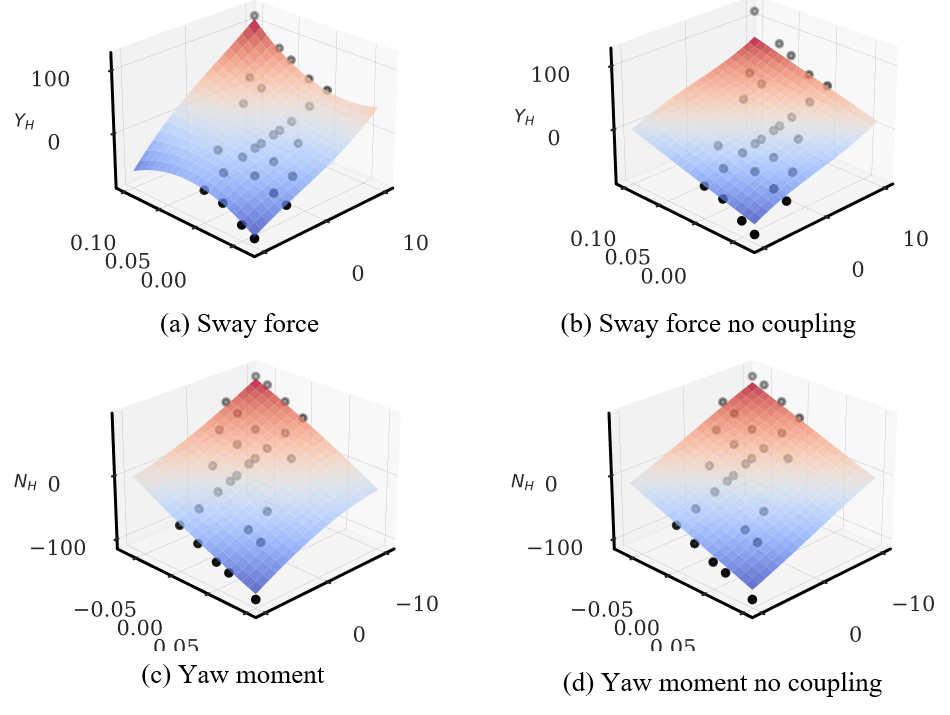
\includegraphics[width=0.8\linewidth]{figures/results_optiwise_vct.YNH.png}
    \caption{Optiwise hull forces during the circle and drift variations with/without the coupling terms, VCT (dots), fitted model (surface).}
    \label{fig:circle_drift_optiwise}
\end{figure}


% % Circle + drift
% \begin{figure}[h]
%      \centering
%      \begin{subfigure}[b]{0.49\textwidth}
%          \centering
%          \includesvg{figures/results_optiwise_VCT.Y_H.svg}
%         \caption{Sway force.}
%         \label{fig:circle_drift_Y_H_optiwise}
%      \end{subfigure}
%      \hfill
%      \begin{subfigure}[b]{0.49\textwidth}
%          \centering         \includesvg{figures/results_optiwise_VCT.Y_H_no_coupling.svg}
%         \caption{Sway force no coupling.}
%         \label{fig:circle_drift_Y_H_no_coupling_optiwise}
%      \end{subfigure}
     
%      \vfill
%      \begin{subfigure}[b]{0.49\textwidth}
%          \centering
%          \includesvg{figures/results_optiwise_VCT.N_H.svg}
%         \caption{Yawing moment.}
%         \label{fig:circle_drift_N_H_optiwise}
%      \end{subfigure}
%      \hfill
%      \begin{subfigure}[b]{0.49\textwidth}
%          \centering
%          \includesvg{figures/results_optiwise_VCT.N_H_no_coupling.svg}
%         \caption{Yawing moment no coupling.}
%         \label{fig:circle_drift_N_H_no_coupling_optiwise}
%      \end{subfigure}
     
%     \caption{Optiwise hull forces during the circle and drift variations with/without the coupling terms, VCT (dots), fitted model (surface).}
%     \label{fig:circle_drift_optiwise}
% \end{figure}